\section{Vorgehensweise}
%Design Thinking / Agile Development als Methode https://dschool.stanford.edu/\\
Die beschriebenen Probleme und Ziele sollen gelöst und erreicht werden mittels der sog. Design Thinking Methode. Bei Design Thinking steht der Empfänger bzw. Nutzer im Fokus. Ein Prozess läuft im weiteren Sinne nach Design Thinking ab, sofern die Methoden von Designern bei Herausforderungen angewendet werden, die über das Aussehen des Produkts hinausgehen.\cite[vgl.]{Patnaik2009} Der Design Thinking Prozess verläuft iterativ und hat fließende Übergänge zwischen den einzelnen Phasen.

\begin{figure}[h!]
	\centering
	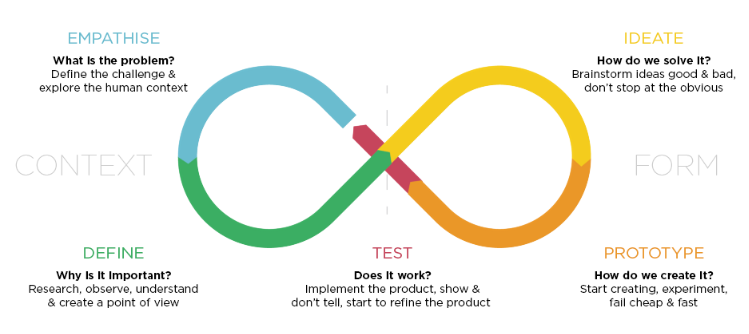
\includegraphics[width=0.9\linewidth]{pictures/Diagram-by-Billy-Loizou-Design-Thinking-blog}
	\caption[Design Thinking Prozess]{Diagram by Billy Loizou - Design Thinking}
	\label{fig:diagram-by-billy-loizou-design-thinking-blog}
\end{figure}

Abbildung \ref{fig:diagram-by-billy-loizou-design-thinking-blog} zeigt das Phasenmodell für Design Thinking. Es wird mit der Verständnisphase gestartet. In dieser Phase soll das eigentliche Problem konkretisiert und in einen Kontext mit dem Nutzer gebracht werden. Mit der Definition legt man das \glqq Warum\grqq~ fest. Dazu \glqq beobachtet\grqq~ und \glqq versteht\grqq~ man das Problem und definiert dann einen Standpunkt aus der Sicht des Nutzers. Anschließend werden durch Innovationsmethoden Ideen evaluiert um das Problem zu lösen. Ein Prototyp wird früh entwickelt um Experimente wagen zu können. In den Prototyp fließen alle Ergebnisse der vorherigen Phase ein. Nach einer kurzen Test Phase geht der Prozess in die nächste Iteration und startet von vorne.\\

Die Auswahl der Softwarehersteller ist nicht Teil dieser Masterarbeit und wurde im Vorfeld auf SAP festgelegt. Mittlerweile agiert SAP als Anbieter einer Cloud Plattform für die unterschiedlichsten Einsatzwecke.\cite{SAP2018} Dazu zählen auch Services wie \ac{baas}, \ac{ml} oder \ac{iot}. Gebündelt werde diese Cloud Services in der Industrie 4.0 Lösung genannt SAP Leonardo. In der Abbildung \ref{fig:sap-leonardo-innovation-system} zeigt SAP schematisch die Architektur von SAP Leonardo auf.

\begin{figure}[h!]
	\centering
	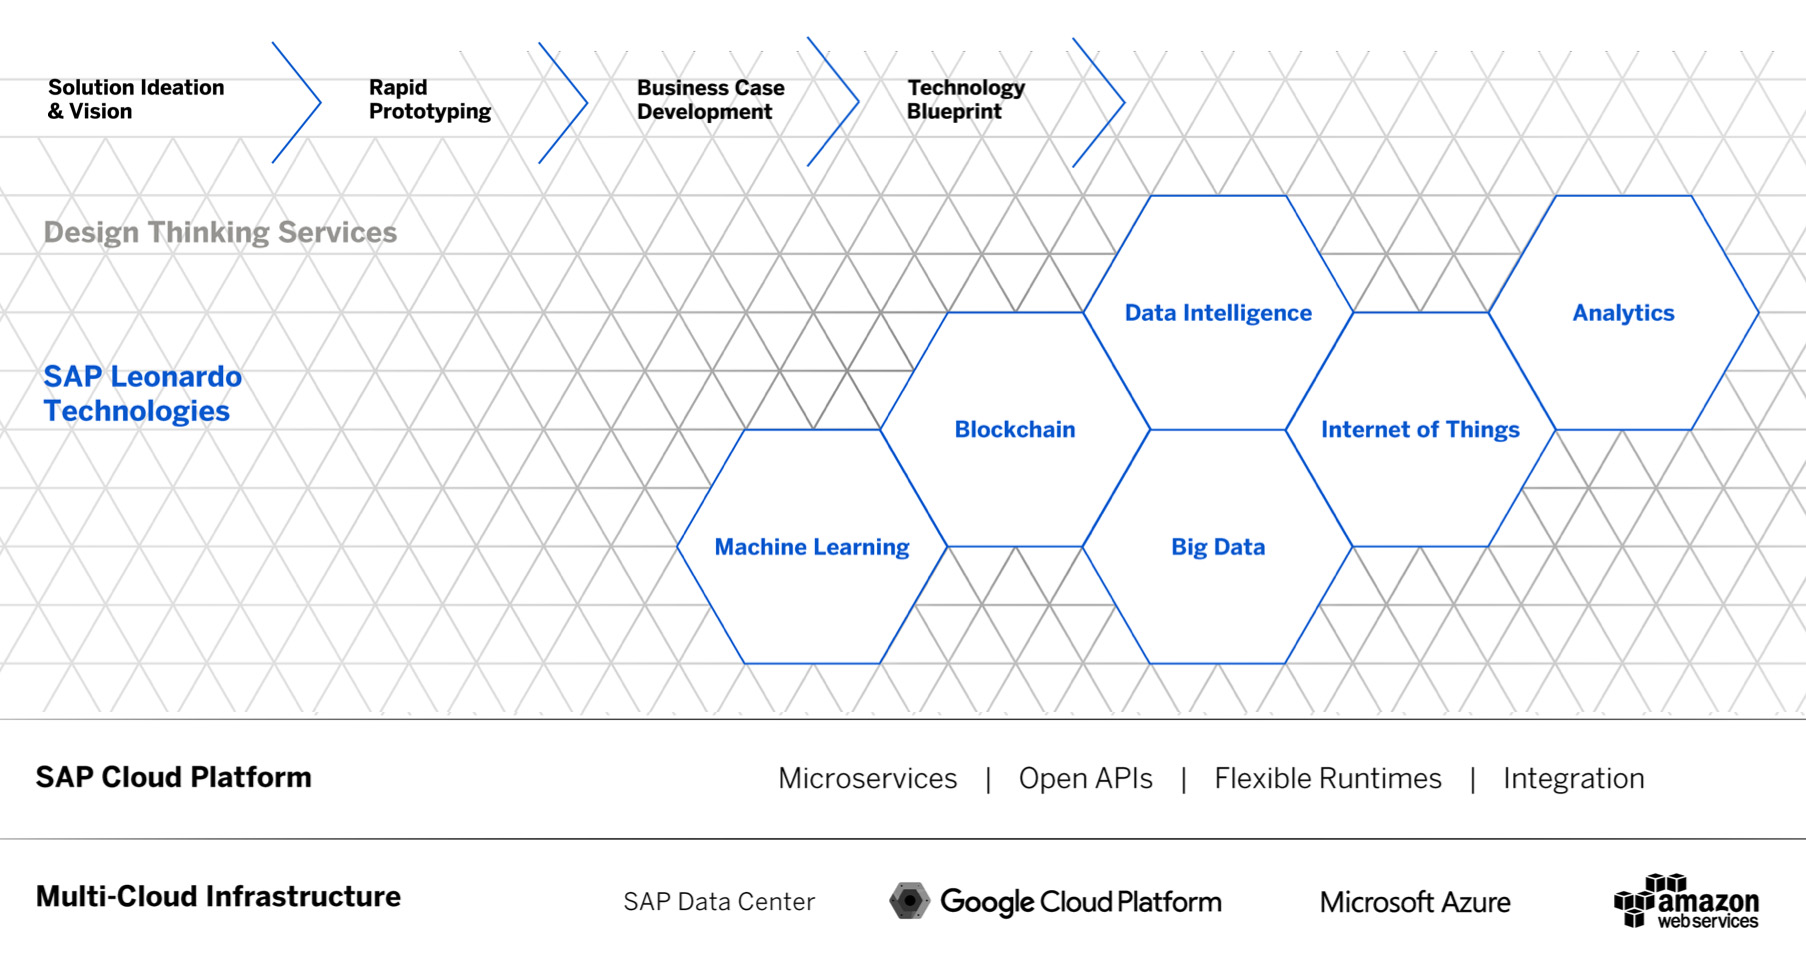
\includegraphics[width=0.9\linewidth]{pictures/sap-leonardo-innovation-system}
	\caption[SAP Leonardo Architektur Übersicht]{SAP Leonardo Architektur Übersicht\cite{Leonardo}}
	\label{fig:sap-leonardo-innovation-system}
\end{figure}

%\begin{itemize}
%	\item Industry Knowledge
%	\begin{itemize}
%	\item Retail
%	\item Consumer Goods
%	\item Manufacturing
%	\item Sports \& Entertainment
%	\item Any industry with Innovation Services
%	\end{itemize}
%
%	\item Software
%	\begin{itemize}
%	\item Cloud
%	\item Big Data
%	\item Machine Learning
%	\item Blockchain
%	\item Analytics
%	\item IoT
%	\end{itemize}
%
%	\item Data Intelligence
%	\begin{itemize}
%	\item 350.000 Companies
%	\item 70\% of Global Business Transactions
%	\end{itemize}
%\end{itemize}

\newpage